\subsection{Angles}

\begin{tcolorbox}[title=Problem 2, breakable]
    Assume that the area of a disc of radius $1$ is equal to the 
    number $\pi$ (approximately equal to $3.14159$...) and that 
    the area of a disc of radius $r$ is $\pi r^2$. \\

    (a) What is the area of a sector in the disc of radius $r$ lying
        between angles of $\theta_1$ and $\theta_2$ degrees, as shown
        in Fig. $5-20 (a)$? \\

    (b) What is the area of the band lying between two circles of radii 
        $r_1$ and $r_2$ as shown in Fig. $5-20 (b)$? \\

    (c) What is the area in the region bounded by angles of $\theta_1$
        and $\theta_2$ degrees and lying between circles of radii $r_1$
        and $r_2$ as shown in Fig. $5-20 (c)$?

    Give your answers in terms of $\pi, \theta_1, \theta_2, r_2, r_1$.
\end{tcolorbox}

\begin{figure}[h]
    \centering
    \includegraphics[width=0.6\textwidth]{images/5_2.png}
\end{figure}

\textbf{Solution 2(a):}

Area $A$ of the sector is 
\[A = \frac{|\theta_2 - \theta_1|}{360} \cdot \pi r_1^2\]

\textbf{Solution 2(b):}

Area $A$ of the band is
\[A = \pi \cdot |r_2^2 - r_1^2|\]

\textbf{Solution 2(c):}

Area $A$ of the region is
\[A = \frac{|\theta_2 - \theta_1|}{360}  \cdot \pi \cdot |r_1^2 - r_2^2|\]

\subsection{The Pythagoras Theorem}

\begin{tcolorbox}[title=Problem 5, breakable]
    What is the length of the diagnol of a rectangle solid whose sides have 
    lengths $a$, $b$, $c$? What if the sides have lengths $ra$, $rb$, $rc$.
\end{tcolorbox}

\begin{figure}[h]
    \centering
    \includegraphics[width=0.6\textwidth]{images/5_3.png}
\end{figure}

\textbf{Solution:}

Let $d$ be the length of the diagnol. Then
\[d = \sqrt{a^2 + b^2 + c^2}\]

If the sides have lengths $ra, rb, rc$ then
\[d = \sqrt{(ra)^2 + (rb)^2 + (rc)^2} = \sqrt{r^2(a^2 + b^2 + c^2)} = r\sqrt{a^2 + b^2 + c^2}\]

\begin{tcolorbox}[title=Problem 9, breakable]
    Write down in detail the ``similar steps'' left to the reader 
    in the proof of the corollary to the Pythagoras theorem. \\

    Previous proof
    \begin{proof}
        Assume first that $d(P, M) = d(Q, M)$. By Pythagoras, we have 
        \begin{align*}
            d(P, O)^2 + d(O, M)^2 
            &= d(P, M)^2 \\
            &= d(Q, M)^2 \\
            &= d(Q, O)^2 + d(O, M)^2
        \end{align*}
        It follows that $d(P, O)^2 = d(Q, O)^2$
        whence $d(P, O) = d(Q, O)$.
    \end{proof}
\end{tcolorbox}

\begin{proof}
    Suppose $d(P, O) = d(Q, O)$.
    By Pythagoras, we have $d(P, O)^2 + d(O, M)^2 = d(P, M)^2$.
    So $d(P, M)^2 - d(O, M)^2 = d(P, O)^2 = d(Q, O)^2 = d(Q, M)^2 - d(O, M)^2$.
    It follows that $d(P, M)^2 = d(Q, M)^2$ so $d(P, M) = d(Q, M)$.
\end{proof}

\begin{tcolorbox}[title=Problem 10, breakable]
    Prove that if $A, B, C$ are the angles of an arbitrary triangle, then
    \[m(A) + m(B) + m(C) = 180\textdegree\]
    by the following method: From any vertex draw the perpendicular to 
    the line of the opposite side. Then use the result already known for 
    right triangles.
\end{tcolorbox}

\begin{figure}[h]
    \centering
    \includegraphics[width=0.6\textwidth]{images/5_4.jpg}
\end{figure}

\begin{proof}
    Consider case $1$. From the figure $m(C) = m(G) + m(F)$.
    The two subtriangles have sums $90\textdegree + m(A) + m(G)$
        and $90\textdegree + m(B) + m(F)$.
    Now by Theorem $1$, $m(A) + m(G) = 90\textdegree$
        and $m(B) + m(F) = 90\textdegree$.
    So $90\textdegree + m(A) + m(G) = 180\textdegree$ then $m(A) = 90\textdegree - m(G)$.
    Similarly, since $90\textdegree + m(B) + m(F)$ then $m(B) = 90\textdegree - m(F)$.
    Then the sum of the angles of the entire 
        triangle is 
    \begin{align*}
        m(A) + m(B) + m(C) 
        &= 90\textdegree - m(G) + 90\textdegree - m(F) + m(C) \\
        &= 180\textdegree -(m(G) + m(F)) + m(C) \\
        &= 180\textdegree - m(C) + m(C) \\
        &= 180\textdegree
    \end{align*}

    Consider case $2$. From the figure $m(D) + m(C) = m(B)$ so $m(C) = m(B) - m(D)$.
    Also $m(F) + m(E) = 180\textdegree$ so $m(E) = 180\textdegree - m(F)$.
    By Theorem $1$, $m(D) + m(F) = 90\textdegree$ and $m(B) + m(A) = 90\textdegree$.
    Then the sum of the angles of the right-most inner triangle is
    \begin{align*}
        m(C) + m(E) + 90\textdegree
        &= m(B) - m(D) + 180\textdegree - m(F) + m(A) \\
        &= m(B) + m(A) + 180\textdegree - (m(D) + m(F)) \\
        &= m(B) + m(A) + 180\textdegree - 90\textdegree \\
        &= m(B) + m(A) + 90\textdegree \\
        &= 90\textdegree + 90\textdegree \\
        &= 180\textdegree
    \end{align*}
\end{proof}

\newpage
\begin{tcolorbox}[title=Problem 11, breakable]
    Show that the area of an arbitrary triangle of heigh $h$ whose base has length $b$
    is $bh/2$. [\emph{Hint:} Decompose the triangle into two right triangles. Distinguish
    between the two pictures in Fig. $5-31$. In one case the area of the triangle is the difference
    of the area of the two right triangles, and in the other case, it is the sum.]
\end{tcolorbox}

\begin{figure}[h]
    \centering
    \includegraphics[width=0.6\textwidth]{images/5_5.jpg}
\end{figure}

\begin{proof}
    Consider case $1$. First note that $b = a + c$.
    By Theorem $2$ (and for the rest of the proof) the area enclosed by the triangle on the right is $\frac{1}{2}ah$.
    The area enclosed by the triangle on the left is $\frac{1}{2}ch$.
    The area of the outer triangle is the sum of the inner triangles
        which is $\frac{1}{2}ch + \frac{1}{2}ah = \frac{1}{2}h(a + c) = \frac{1}{2}bh$.

    Consider case $2$. The area enclosed by the outer triangle is $\frac{1}{2}h(a + b)$.
    Then, the area enclosed by the right inner triangle is the area enclosed 
        by the outer triangle minus the left inner triangle which is 
            $\frac{1}{2}h(a + b) - \frac{1}{2}ha = \frac{1}{2}h(a + b - a) = \frac{1}{2}bh$.
\end{proof}

\newpage
\begin{tcolorbox}[title=Problem 12, breakable]
    (a) Show that the length of the hypotenuse of a right triangle is $\ge$ the length 
        of a leg. \\

    (b) Let $P$ be a point and $L$ a line. Show that the smallest value for the distances 
        $d(P, M)$ between $P$ and points $M$ on the line is the distance $d(P, Q)$,
        where $Q$ is the point of the intersection between $L$ and teh line through $P$,
        perpendicular to $L$.
\end{tcolorbox}

\begin{figure}[h]
    \centering
    \includegraphics[width=0.6\textwidth]{images/5_12.png}
\end{figure}

\begin{proof}
    Let $a$,$b$ be the legs of a right triangle and $c$ be the hypotenuse.
    By Pythagoras's Theorem we know that $c^2 = a^2 + b^2$.
    Since $b^2 \ge 0$ it follows that $c^2 \ge a^2$.
    Since $c, a \ge 0$ it follows that $c \ge a$.
    Similarly, $c^2 \ge b^2$ implies $c \ge b$.  
    Therefore the hypotenuse $c$ is greater than or equal to each leg $a, b$.
\end{proof}

\begin{proof}
    Let $c$ be the hypotenuse of the right triangle formed by points $P$, $Q$, and $M$, 
    where $Q$ is the point on the line $L$ such that $\overline{PQ}$ is perpendicular to $L$, 
    and $M$ is any other point on $L$.  
    The hypotenuse of this triangle is $d(P, M)$, and we want to choose $M$ to minimize this distance.  
    By the Pythagorean Theorem,  
    \[
        d(P, M)^2 = d(P, Q)^2 + d(Q, M)^2.
    \]
    The smallest value for $d(Q, M)^2$ is $0$, which occurs if and only if $Q = M$.  
    So when $Q = M$, we have $d(P, M) = d(P, Q)$.  
    Therefore, the smallest distance from $P$ to a point on the line $L$ is $d(P, Q)$.
\end{proof}

\newpage
\begin{tcolorbox}[title=Problem 13, breakable]
    This exercize asks you to derive some standard properties of angles from 
    elementary geometry. They are used very commonly. We refer to the following figures. \\

    (a) In Fig. $5-33$(a), you are given two parallel lines $L_1, L_2$ and a line $K$
        which intersects them at points $P$ and $P'$ as shown. Let $A$ and $B$ then 
        be angles which $K$ makes with $L_1$ and $L_2$ respectively, as shown.
        Prove that $m(A) = m(B)$. [\emph{Hint}: Draw a line from a point of $K$ above 
        $L_1$ and $L_2$. Then use the fact that the sum of the angles of a right triangle 
        has $180\textdegree$.] \\

    (b) In Fig. $5-33$(b), you are given $L_1, L_2$ and $K$ again. Let $B$ and $B'$ be 
        the alternate angles formed by $K$ and $L_1$, $L_2$ respectively, as shown.
        Prove that $m(B) = m(B')$. (Actually, all you need to do here is refer 
        to the appropriate portion of the text. Which is it?) \\

    (c) Let $K, L$ be two lines as shown on Fig. $5-33$(c). Prove that the opposite 
        angles $A$ and $A'$ as shown have equal measure.
\end{tcolorbox}

\begin{figure}[h]
    \centering
    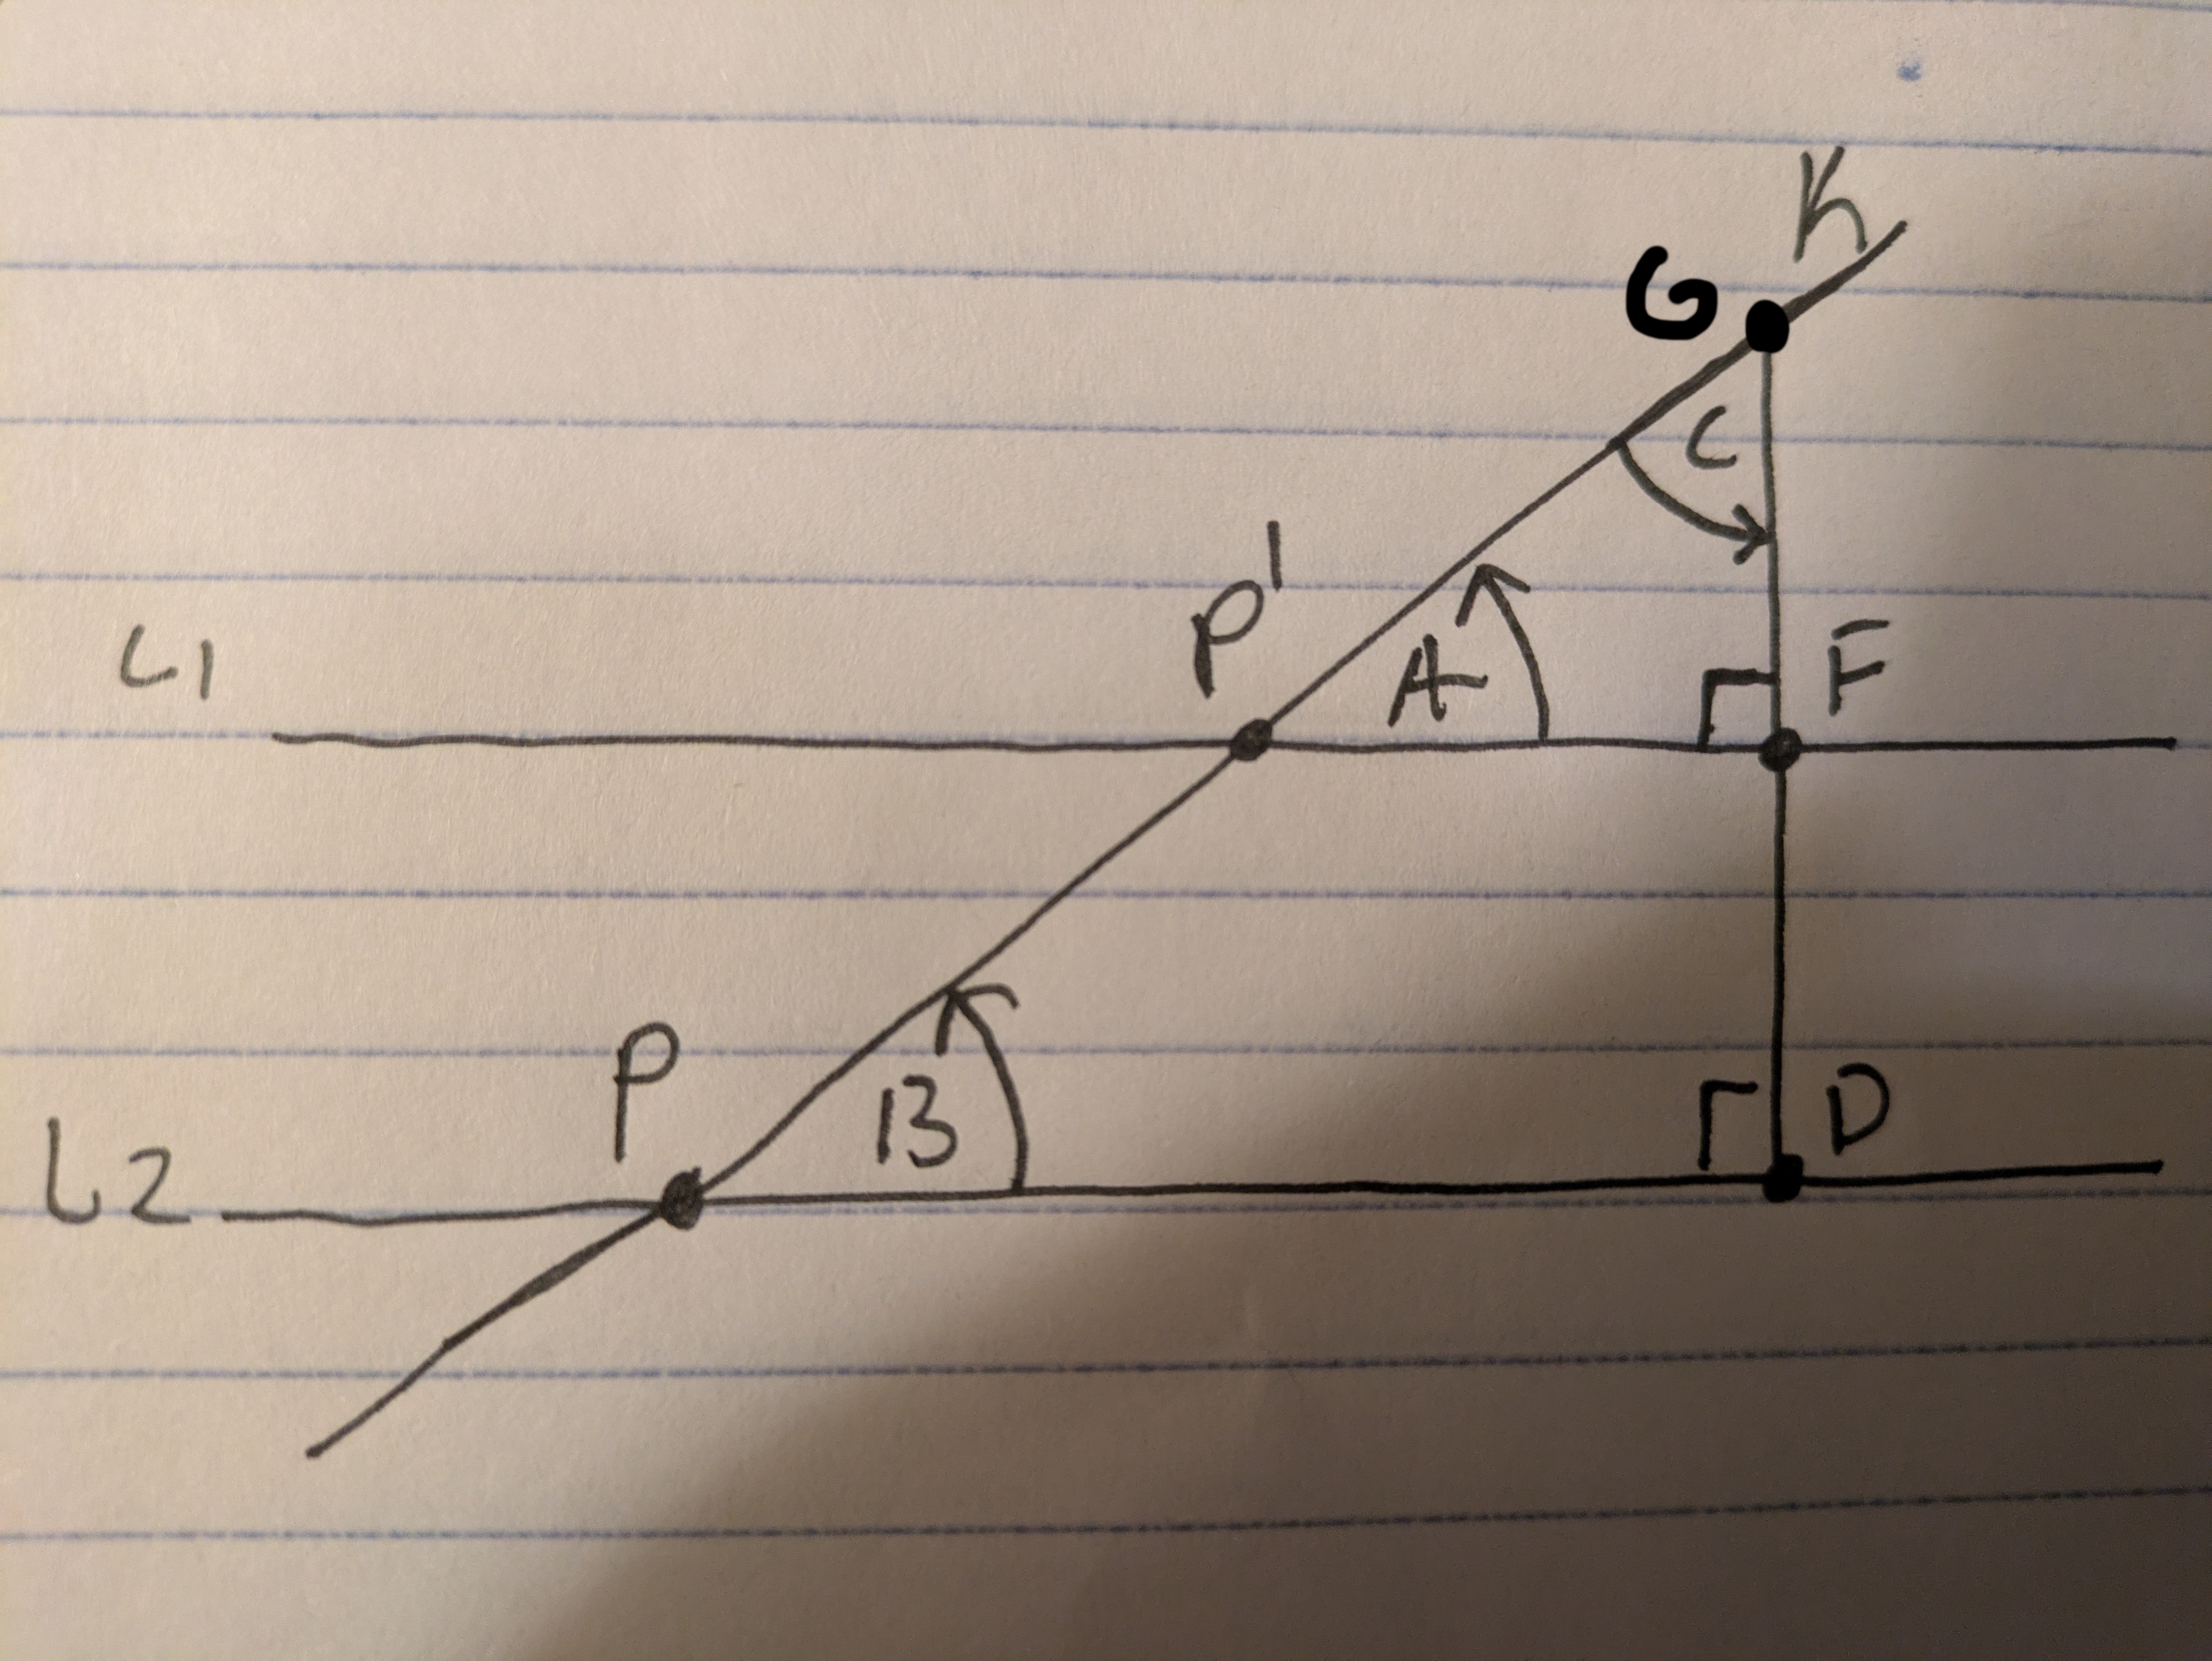
\includegraphics[width=0.6\textwidth]{images/5_5_a.jpg}
\end{figure}

\begin{figure}[h]
    \centering
    \includegraphics[width=0.6\textwidth]{images/5_again.png}
\end{figure}

\begin{figure}[h]
    \centering
    \includegraphics[width=0.6\textwidth]{images/lets_go.png}
\end{figure}

\begin{proof}
    Refer to the figure. Consider the areas enclosed by the right triangles 
        $\triangle P'FG$ and $\triangle PDG$.
    By Problem $10$, the degrees of $\triangle P'FG$ is $90\textdegree + m(A) + m(C) = 180\textdegree$.
    Similarly, the degress of $\triangle PDG$ is $90\textdegree + m(B) + m(C) = 180\textdegree$.
    Then $90\textdegree + m(A) + m(C) = 90\textdegree + m(B) + m(C)$
        and it follows that $m(A) = m(B)$.
\end{proof}

\begin{proof}
    Refer to the text. Then let the parallel segments formed by points $Q, P$ and $N, M$
        be the parallel lines $L_1$, $L_2$. Also let $B$ be the $B$ in our problem.
    Finally, let $\angle NQM$ be $m(B')$.
    It then follows from the text that $m(B) = m(B')$.
\end{proof}

\begin{proof}
    Refer to the figure. Line $D$ is parallel to line $K$.
    The measure of the green angle is equal to $m(A)$ by Problem $13$(b).
    Then $m(A') = m(A)$ by Problem $13$(a).
\end{proof}
